\documentclass[11pt]{article}
\usepackage[scaled=0.92]{helvet}
\usepackage{geometry}
\geometry{letterpaper,tmargin=1in,bmargin=1in,lmargin=1in,rmargin=1in}
\usepackage[parfill]{parskip} % Activate to begin paragraphs with an empty line rather than an indent %\usepackage{graphicx}
\usepackage{amsmath,amssymb, mathrsfs,  mathtools, dsfont}
\usepackage{tabularx}
\usepackage{tikz-cd}
\usepackage[font=footnotesize,labelfont=bf]{caption}
\usepackage{graphicx}
\usepackage{xcolor}
%\usepackage[linkbordercolor ={1 1 1} ]{hyperref}
%\usepackage[sf]{titlesec}
\usepackage{natbib}
\usepackage{../../Tianpei_Report}

%\usepackage{appendix}
%\usepackage{algorithm}
%\usepackage{algorithmic}

%\renewcommand{\algorithmicrequire}{\textbf{Input:}}
%\renewcommand{\algorithmicensure}{\textbf{Output:}}



\begin{document}
\title{Lecture 8: Vector Fields}
\author{ Tianpei Xie}
\date{Oct. 16th., 2022}
\maketitle
\tableofcontents
\newpage
\section{Vector Fields on Manifolds}
\subsection{Definitions}
\begin{itemize}
\item \begin{definition}
If $M$ is a smooth manifold with or without boundary, a \underline{\emph{\textbf{vector field}}} on $M$ is a \emph{\textbf{section}} of the map $\pi: TM \rightarrow M$. More concretely, a \emph{vector field} is a \emph{\textbf{continuous}} map $X: M \rightarrow TM$, usually written $p \mapsto X_p$, with the property that
\begin{align}
\pi \circ X = \text{Id}_{M}, \label{eqn: section_definition}
\end{align} or \emph{equivalently}, $X_p \in T_{p}M$ for each $p \in M$. 
\end{definition}

\begin{figure}
\begin{minipage}[htb]{1\linewidth}
  \centering
  \centerline{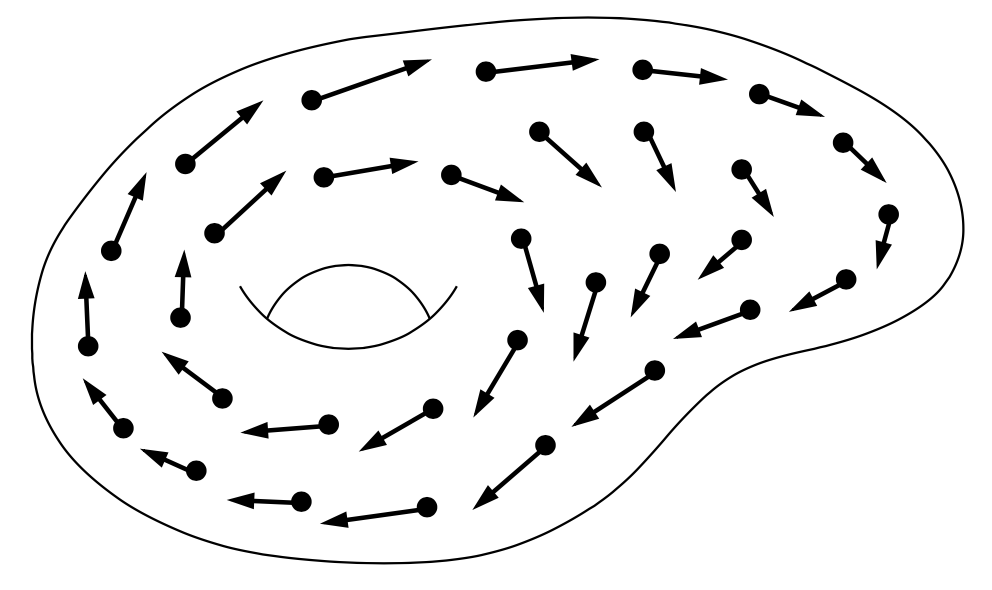
\includegraphics[scale = 0.5]{vector_fields_2.png}}
\end{minipage}
\caption{\footnotesize{\textbf{A vector field \citep{lee2003introduction}}}}
\label{fig: vector_fields}
\end{figure}

\item \begin{remark}
We write the \emph{\textbf{value of $X$ at $p$}} as $X_p$ instead of $X(p)$ to be consistent with our notation for elements of the tangent bundle, as well as to avoid conflict with the notation $v(f)$ for the action of a vector on a function.
\end{remark}

\item \begin{remark}
You should visualize a vector field on $M$ in the same way as you visualize vector fields in Euclidean space: as an arrow attached to each point of $M$, chosen to be tangent to $M$ and to \emph{\textbf{vary continuously from point to point}} (Fig. \ref{fig: vector_fields}).
\end{remark}

\item \begin{remark}
We can compare several related concepts:
\begin{itemize}
\item \emph{\textbf{Tangent vector}} $v \in T_{p}M$ is both a \emph{geometric tangent vector}, i.e. the tangent direction for some curve on $M$ passing $p$, and a \emph{derivation} at $p$ defined on $\cC^{\infty}(M)$ that satisfies the product rule. For the latter case, $v$ is a \emph{linear functional} that act on functions $f \in \cC^{\infty}(M)$.  $v(f)$ induces the \emph{directional derivatives} of $f$ along $v$ and \emph{derivation at $p$}.

\item The \emph{\textbf{differential}} of $F: M\rightarrow N$ at $p$, $dF_{p}$, is a \emph{linear operator} from $T_{p}M$ to $T_{p}N$. $dF_{p}$ maps a \emph{tangent vector} at $p$ in $M$ to a \emph{tangent vector} at $F(p)$ in $N$. Since tangent vectors are functions, $dF_{p}$ is also a linear functional if $F: M\rightarrow \bR$. $dF_{p}(v) \in T_{F(p)}N$ can act on a function on $N$ to have $dF_{p}(v)(f)$.

\item The \emph{\textbf{vector field}} $X$ is a \emph{continuous} map from a point $p \in M$ to a \emph{tangent vector} $X_p = v \in T_{p}M$. Thus for smooth function $f$ on $M$, $X_{p}f$ is a real-value, i.e. the directional derivative of $f$ along $v=X_{p}$.   A vector field $X$ is also  \emph{\textbf{a derivation operator}} on $\cC^{\infty}(M)$. It maps a \emph{smooth function} $f$ to a \emph{new smooth function} $Xf$ which at each point is $X_{p}f$. A vector field is a \emph{global generalization} of a tangent vector. 
% a \emph{global} concept associated with the tangent bundle $TM$ as opposed to a tangent vector $v \in T_{p}M$. $X(f)$ defines the derivation (not just for one point) on the manifold $M$, which itself is a function of $p\in M$. The image of a vector field covers the entire tangent bundle, which is a \emph{global concept}.
\end{itemize}
\end{remark}

\item \begin{definition}
When the map $X: M \rightarrow TM$ is \emph{smooth} and the tangent bundle $TM$ is given a \emph{smooth manifold structure},  $X$ is a \textbf{\emph{smooth vector field}}. 

In addition, for some purposes it is useful to consider maps from $M$ to $TM$ that would be vector fields except that they \emph{might not be continuous}. A \emph{\textbf{rough vector field}} on $M$ is a (\emph{not necessarily continuous}) map $X: M \rightarrow TM$ satisfying \eqref{eqn: section_definition}.
\end{definition}

\item \begin{definition}
Just as for functions, if $X$ is a vector field on $M$, the \emph{\textbf{support of $X$}} is defined to be \emph{the closure of the set} $\set{p \in M: X_p \neq 0}$. A vector field is said to be \emph{\textbf{compactly supported}} if its support is a \emph{compact set}.
\end{definition}

\item \begin{remark} (\emph{\textbf{Coordinate Representation of Vector Field At a Point}})\\
Suppose $M$ is a smooth $n$-manifold (with or without boundary). If $X: M \rightarrow TM$ is a \emph{rough vector field} and $(U, (x^i)) $ is any \emph{smooth coordinate chart} for $M$, we can write the \emph{\textbf{value} of $X$ at any point $p \in U$} in terms of the coordinate basis vectors:
\begin{align}
X_{p} &= X^{i}(p)\,\partdiff{}{x^{i}}\Bigr|_{p}.  \label{eqn: vector_fields_at_p_coordinate_expansion}
\end{align} 
This defines \textbf{\emph{$n$ functions}} $X^i: U \rightarrow \bR$, called the \emph{\textbf{component functions}} of $X$ in the given chart.
\end{remark}

\item Note that a \emph{component function} is a real-value function on neighborhood $U \subseteq M$. It is necessary to distinguish \eqref{eqn: vector_fields_at_p_coordinate_expansion} from the coordinate representation of tangent vector $v\in T_{p}M$
\begin{align*}
v &= v^{i}\,\partdiff{}{x^{i}}\Bigr|_{p},
\end{align*} where $v^{i} \in \bR$ is a fixed constant.

\item 
\begin{proposition}\label{prop: vector_field_smooth_condition} (\textbf{Smoothness Criterion for Vector Fields}) \citep{lee2003introduction} \\
Let $M$ be a smooth manifold with or without boundary, and let $X: M \rightarrow TM$ be a rough vector field. If $(U, (x^i))$ is any smooth coordinate chart on $M$, then the \textbf{restriction} of $X$ to $U$ is \textbf{smooth} if and only if its \textbf{component functions} with respect to this chart are \textbf{smooth}.
\end{proposition}

\item \begin{definition}
If $M$ is a smooth manifold with or without boundary and $A \subseteq M$ is an arbitrary subset, \emph{\textbf{a vector field along $A$}} is a \emph{continuous} map $X: A \rightarrow TM$ satisfying $\pi \circ X = \text{Id}_A$ (or in other words $X_p \in TpM$  for each $p \in A$). 

We call it \emph{\textbf{a smooth vector field along $A$}} if for each $p \in A$, there is a \emph{neighborhood} $V$ of $p$ in $M$ and a \emph{smooth vector field} $\widetilde{X}$ on $V$ that agrees with $X$ on $V \cap A$.
\end{definition}

\item \begin{lemma} (\textbf{Extension Lemma for Vector Fields}). \citep{lee2003introduction} \\
Let $M$ be a smooth manifold with or without boundary, and let $A \subseteq M$ be a closed subset. Suppose $X$ is a smooth vector field along $A$. Given any open subset $U$ containing $A$, there exists a \textbf{smooth global vector field} $\widetilde{X}$ on $M$ such that $\widetilde{X}|_{A} = X$ and $\text{supp}\,\widetilde{X} \subseteq U$.
\end{lemma}

\item As an important special case, \emph{\textbf{any vector} at a point can be \textbf{extended} to a \textbf{smooth vector field} on the \textbf{entire manifold}}.
\begin{proposition}\label{prop: vector_field_extend_from_one_vector}
Let $M$ be a smooth manifold with or without boundary. Given $p \in M$ and $v \in T_{p}M$, there is a smooth global vector field $X$ on $M$ such that $X_p  = v$.
\end{proposition}

\item \begin{remark} (\emph{\textbf{The Space of all Vector Fields on a Manifold is a Vector Space}})\\
If $M$ is a smooth manifold with or without boundary, it is standard to use the notation $\mathfrak{X}(M)$ to denote \emph{\textbf{the set of all smooth vector fields on M}}. 

\underline{\emph{$\mathfrak{X}(M)$ is a \textbf{vector space}} under pointwise addition and scalar multiplication}:
\begin{enumerate}
\item For any $a, b \in \bR$ and any $X, Y \in \mathfrak{X}(M)$,
\begin{align*}
(a\,X + b\,Y)_{p} &= a\,X_{p} + b\,Y_{p}.
\end{align*}
\item The \emph{zero element} of this vector space is the \emph{\textbf{zero vector field}}, whose value at each $p \in M$ is $0 \in T_{p}M$.
\end{enumerate}

In addition, \emph{smooth vector fields} can be multiplied by \emph{smooth real-valued functions}: if $f \in \cC^{\infty}(M)$ and $X \in \mathfrak{X}(M)$, we define $fX: M \rightarrow TM$ by
\begin{align*}
(fX)_p &= f(p)\, X_p.
\end{align*}
\end{remark}

\item \begin{proposition}
Let $M$ be a smooth manifold with or without boundary.
\begin{enumerate}
\item If $X$ and $Y$ are smooth vector fields on $M$ and $f,g \in \cC^{\infty}(M)$, then $fX + gY $ is a smooth vector field.
\item $\mathfrak{X}(M)$ is a \textbf{module} over the \textbf{ring} $\cC^{\infty}(M)$.
\end{enumerate}
\end{proposition}

\item \begin{remark} (\emph{\textbf{Coordinate Representation of Vector Field}})\\
We can generalize the formula \eqref{eqn: vector_fields_at_p_coordinate_expansion} as the coordinate representation of the vector field $X$
\begin{align}
X &= X^{i}\,\partdiff{}{x^{i}}.  \label{eqn: vector_fields_coordinate_expansion}
\end{align}  where $(\partdiff{}{x^{i}})$ are \emph{the coordinate vector fields}, which are \emph{\textbf{basis}} for $\mathfrak{X}(M)$ and $X^i$ is the $i$-th component function of $X$ in the given coordinates.

In partial differential equations (PDEs), we usually write \eqref{eqn: vector_fields_coordinate_expansion} in \emph{dot-product form}
\begin{align}
&X = \mb{X} \cdot \nabla = \sum_{i=1}^{n}X^{i}\,\partdiff{}{x^{i}} \label{eqn: vector_fields_coordinate_dot_product}\\
&\quad \text{where }\mb{X} = [X^{1}, \ldots, X^{n}], \quad \nabla := \paren{\partdiff{}{x^{1}}, \ldots, \partdiff{}{x^{n}}}.  \nonumber
\end{align} $\nabla$ (\emph{the nabla symbol}) is also called \emph{\textbf{gradient operator}}.
\end{remark}

\item Note that we need to distinguish the difference between the \emph{\textbf{coordinate vector}} $\partdiff{}{x^{i}}|_{p}$ in tangent space $T_{p}M$ and the \emph{\textbf{coordinate vector fields}} $\partdiff{}{x^{i}}$ as latter is a smooth function on $M$. 
\end{itemize}

\subsection{Examples of Smooth Vector Fields}
\begin{itemize}
\item 
\begin{example} (\emph{\textbf{Coordinate Vector Fields}}). \\
If $(U, (x^i))$ is any \emph{smooth} \emph{chart} on $M$, the assignment
\begin{align*}
p \mapsto \partdiff{}{x^{i}}\Bigr|_{p}
\end{align*} determines a \emph{vector field} on $U$, called \underline{\emph{\textbf{the $i$-th coordinate vector field}}} and denoted by $\partdiff{}{x^{i}}$ (without $p$ since it is now a function of $p$). It is \emph{\textbf{smooth}} because its component functions are \emph{constants}.
\end{example}

\item \begin{example} (\emph{\textbf{The Euler Vector Field}}). \\
The \emph{vector field} $V$ on $\bR^n$ whose value at $x \in \bR^n$ is
\begin{align*}
V_x & = x^{1}\,\partdiff{}{x^{1}}\Bigr|_{x} + \ldots + x^{n}\,\partdiff{}{x^{n}}\Bigr|_{x}.
\end{align*} is \emph{\textbf{smooth}} because its coordinate functions are \emph{linear}. It \emph{vanishes} at the origin, and points \emph{radially \textbf{outward} everywhere else}. It is called \emph{\textbf{the Euler vector field}} because of its appearance in \emph{Euler’s homogeneous function theorem}.
\end{example}

\item \begin{example} (\emph{\textbf{The Angle Coordinate Vector Field on the Circle}}).\\
Let $\theta$ be any \emph{angle coordinate} on a proper open subset $U \subseteq \bS^1$, and let $\frac{d}{d\theta}$ denote the corresponding coordinate vector field. Because any other angle coordinate $\widetilde{\theta}$ differs from $\theta$ by an additive constant in a neighborhood of each point, the transformation law for coordinate vector fields (i.e. the change of coordinate law) shows that $\frac{d}{d\theta} = \frac{d}{d\widetilde{\theta}}$ on their common domain. 

For this reason, there is a \emph{\textbf{globally defined vector field}} on $\bS^1$ whose coordinate representation is $\frac{d}{d\theta}$  with respect to any angle coordinate. It is a \emph{\textbf{smooth}} vector field because its component function is \emph{constant} in \emph{any such chart}. We denote this global vector field by $\frac{d}{d\theta}$, even though, strictly speaking, it cannot be considered as a coordinate vector field on the entire circle at once.
\end{example}

\item \begin{example} (\emph{\textbf{Angle Coordinate Vector Fields on Tori}}). \\
On the $n$-dimensional torus $\mathbb{T}^n$, choosing an angle function $\theta^i$ for the $i$-th circle factor, $i = 1,\ldots,n$, yields local coordinates $(\theta^1,\ldots,\theta^n)$ for $\mathbb{T}^n$. An analysis similar to that of the previous example shows that the coordinate vector fields $\frac{d}{d\theta^1}, \ldots, \frac{d}{d\theta^n}$ are \emph{\textbf{smooth}} and \emph{\textbf{globally defined}} on $\mathbb{T}^n$.
\end{example}

\item \begin{example} (\emph{\textbf{Restriction of Vector Field on Open Submanifold}}) \\
If $U \subseteq M$ is open, the fact that $T_{p}U$ is \emph{naturally identified} with $T_{p}M$ for each $p \in U$ (See Chapter 3) allows us to identify $TU$ with the open subset $\pi^{-1}(U) \subseteq TM$. Therefore, a vector field on $U$ can be thought of either as a map from $U$ to $TU$ or as a map from $U$ to $TM$ whichever is more convenient.

If $X$ is a \emph{vector field} on $M$, \emph{its restriction $X|_{U}$ is a vector field on $U$}, which is \emph{smooth if $X$ is}.
\end{example}
\end{itemize}

\subsection{Local and Global Frames}
\begin{itemize}
\item Coordinate vector fields in a smooth chart provide a convenient way of representing vector fields, because their values form a basis for the tangent space at each point. However, they are not the only choices. 

\item \begin{definition}
Suppose $M$ is a smooth $n$-manifold with or without boundary. An \emph{ordered $k$-tuple} $(X_1, \ldots, X_k)$ of \emph{\textbf{vector fields}} defined on some subset $A \subseteq M$ is said to be \textit{\textbf{linearly independent}} if $(X_1|_{p}, \ldots, X_k|_{p})$ is a \emph{linearly independent} $k$-tuple in $T_{p}M$ for each $p \in A$, and is said to \emph{\textbf{span the tangent bundle}} if the $k$-tuple $(X_1|_{p},\ldots,X_k|_{p})$ spans $T_{p}M$ at each $p \in A$. 
\end{definition}

\item \begin{definition}
A \underline{\emph{\textbf{local frame}}} for $M$ is \emph{an ordered $n$-tuple of \textbf{vector fields}} $(E_1,\ldots,E_n)$ defined on an \textbf{open subset} $U \subseteq M$ that is \emph{\textbf{linearly independent}} and \emph{\textbf{spans the tangent bundle}}; thus the vectors $(E_1|_{p},\ldots,E_n|_{p})$ form a basis for $T_{p}M$ at each $p \in U$.

$(E_1,\ldots,E_n)$ is called a \underline{\emph{\textbf{global frame}}} if $U = M$, and a \emph{\textbf{smooth frame}} if each of the vector fields $E_i$ is \emph{smooth}.
\end{definition} We often use the shorthand notation $(E_i)$ to denote a frame $(E_1,\ldots,E_n)$. 

\item  If $M$ has dimension $n$, then to check that an ordered $n$-tuple of vector fields $(E_1,\ldots,E_n)$ is a local frame, it suffices to check either that \emph{it is linearly independent} \textbf{or} that \emph{it spans the tangent bundle}.

\item 
\begin{example} (\emph{\textbf{Local and Global Frames}}).
\begin{itemize}
\item The \emph{\textbf{standard coordinate vector fields}} $(\partdiff{}{x^{i}})$ form a \textbf{\emph{smooth global frame}} for $\bR^n$.
\item If $(U, (x^i))$ is any smooth coordinate chart for a smooth manifold $M$ (possibly with boundary), then the \emph{coordinate vector fields} form a \emph{\textbf{smooth local frame}} $(\partdiff{}{x^{i}})$ on $U$, called a \underline{\emph{\textbf{coordinate frame}}}. \emph{Every point of $M$} is in the domain of such a local frame.
\item The \emph{\textbf{angle coordinate vector field}} $\frac{d}{d\theta}$ constitutes a \emph{smooth global frame} for the circle $\bS^1$.
\item The $n$-tuple of vector fields $(\frac{d}{d\theta^{i}})$ is a \emph{smooth global frame} for the $n$-torus $\mathbb{T}^{n}$.
\end{itemize}
\end{example}

\item \begin{proposition} (\textbf{Completion of Local Frames}).\\
Let $M$ be a smooth $n$-manifold with or without boundary.
\begin{enumerate}
\item If $(X_1,\ldots,X_k)$ is a linearly independent $k$-tuple of smooth vector fields on an \textbf{open subset} $U \subseteq M$, with $1 \le k < n$, then for each $p \in U$ there exist smooth vector fields $X_{k+1},\ldots,X_{n}$ in a \textbf{neighborhood} $V$ of $p$ such that $(X_1,\ldots,X_n)$ is a smooth local frame for $M$ on $U \cap V$.
\item If $(v_1, \ldots, v_k)$ is a linearly independent $k$-tuple of vectors in $T_{p}M$ for some $p \in M$, with $1 \le k \le n$, then there exists a \textbf{smooth local frame} $(X_i)$ on a \textbf{neighborhood} of $p$ such that $X_i|_{p}  = v_i$ for $i = 1,\ldots,k$.
\item If $(X_1,\ldots,X_n)$ is a linearly independent $n$-tuple of smooth vector fields along a \textbf{closed subset} $A \subseteq M$, then there exists a \textbf{smooth local frame} $(\widetilde{X}_1,\ldots, \widetilde{X}_n)$ on some neighborhood of $A$ such that $\widetilde{X}_i|_{A}  = X_i$ for $i = 1,\ldots,n$.
\end{enumerate}
\end{proposition}

\item \begin{definition}
A $k$-tuple of vector fields $(E_1,\ldots,E_k)$ defined on some subset $A \subseteq \bR^n$ is said to be \emph{\textbf{orthonormal}} if for each $p \in A$, the vectors $(E_1|_{p},\ldots,E_k|_{p})$ are \emph{\textbf{orthonormal}} with respect to the Euclidean dot product (where we identify $T_{p}\bR^n$ with $\bR^n$ in the usual way). 

A \emph{(local or global) frame} consisting of \emph{orthonormal vector fields} is called an \emph{\textbf{orthonormal frame}}.
\end{definition}

\item \begin{lemma}\label{lemma: gram_schmidt} (\textbf{Gram-Schmidt Algorithm for Frames}). \\
Suppose $(X_j)$ is a smooth local frame for $T \bR^n$ over an open subset $U \subseteq \bR^n$. Then there is a smooth orthonormal frame $(E_j)$ over $U$ such that $\text{span}(E_1|_{p},\ldots, E_j|_{p}) = \text{span}(X_1|_{p},\ldots, X_j|_{p})$ for each $j = 1,\ldots,n$ and each $p \in U$.
\end{lemma}

\item Although \emph{smooth local frames} are plentiful, \emph{global ones} are not.
\begin{definition}
A smooth manifold with or without boundary is said to be \emph{\textbf{parallelizable}} if it admits a \textbf{smooth global frame}.
\end{definition}

\item 
\begin{example} These are some examples of parallizable or non-parallizable manifolds:
\begin{itemize}
\item $\bR^{n}$, $\bS^{1}$ and $\mathbb{T}^{n}$ are all \emph{parallelizable manifold}.
\item \emph{All \textbf{Lie groups}} are \emph{parallelizable}.
\item Most smooth manifolds are \emph{not parallelizable}. The simplest example of a \emph{nonparallelizable manifold} is $\bS^2$. (In fact, $\bS^{1}$, $\bS^{3}$ and $\bS^{7}$ are the \emph{\textbf{only}} spheres that are parallelizable.)
\end{itemize}
\end{example}
\end{itemize}

\subsection{Vector Fields as Derivations of $\cC^{\infty}(M)$}
\begin{itemize}
\item An essential property of vector fields is that they define \emph{\textbf{operators}} on the space of smooth real-valued functions.

\begin{definition}
 If $X \in \mathfrak{X}(M)$ and $f$ is a smooth real-valued function defined on an open subset $U \subseteq M$, we obtain a new function $Xf:  U \rightarrow \bR$, defined
by 
\begin{align*}
(X\,f)_{p} &=  X_{p}\,f
\end{align*} Note that $v\,f \equiv v(f)$ as we omit the parenthesis.
\end{definition}

\item \begin{remark}
Be careful not to confuse the notations $fX$ and $Xf$:
\begin{itemize}
\item  the former $fX$ is \emph{\textbf{the smooth vector field}} on $U$ obtained by multiplying $X$ by $f$,
\item  while the latter $Xf$ is \emph{\textbf{the real-valued functio}n} on $U$ obtained by \emph{applying} the vector field $X$ to the smooth function $f$.
\end{itemize}
\end{remark}

\item \begin{remark}
Because the action of a tangent vector on a function is determined by the values of the function in an arbitrarily small neighborhood, it follows that $Xf$ is \emph{\textbf{locally determined}}. In particular,  for any open subset $V \subseteq U$, 
\begin{align}
(X\,f)\bigr|_{V} &= X\paren{f \bigr|_{V}}.  \label{eqn: local_vector_field_on_function}
\end{align}
\end{remark}

\item \begin{proposition}
Let $M$ be a smooth manifold with or without boundary, and let $X: M \rightarrow TM$ be a \textbf{rough vector field}. The following are equivalent:
\begin{enumerate}
\item  $X$ is smooth.
\item  For \textbf{every} $f \in \cC^{\infty}(M)$,  the function $Xf$ is smooth on $M$.
\item For \textbf{every open subset} $U \subseteq M$ and every $f \in \cC^{\infty}(U)$, the function $Xf$ is smooth on $U$.
\end{enumerate}
\end{proposition}

\item \begin{definition}
Define a map $X: \cC^{\infty}(M) \rightarrow \cC^{\infty}(M)$ is called a \underline{\emph{\textbf{derivation}}} (as distinct from a \emph{derivation at p}, defined in Chapter 3) if it is \textbf{linear} over $\bR$ and satisfies the \emph{Leibnitz rule}
\begin{align}
X(fg) &= f\, X(g) + g\, X(f),  \qquad \forall\,\, f,g \in \cC^{\infty}(M) \label{eqn: derivation_vector_fields}
\end{align}
\end{definition}

\item \begin{remark}
As the tangent vector itself is a \emph{\textbf{linear functional}} on $\cC^{\infty}(M)$, the vector field $X$ is a \emph{\textbf{linear operator}} that maps a function to another function on $\cC^{\infty}(M)$. The \emph{\textbf{value} of function} $Xf$ at $p$ is \emph{the directional derivative} of $f$ \emph{along with} $X(p)$ at point $p$.
\end{remark}

\item The next proposition shows that \emph{derivations} of $\cC^{\infty}(M)$ can be identified with smooth vector fields:
\begin{proposition}
Let $M$ be a smooth manifold with or without boundary. A map $D: \cC^{\infty}(M) \rightarrow \cC^{\infty}(M)$ is a \textbf{derivation} \textbf{if and only} if it is of the form $Df = Xf$ for \textbf{some smooth vector field} $X \in \mathfrak{X}(M)$.
\end{proposition}

\item \begin{remark}
Because of this result, we sometimes \emph{\textbf{identify}} \emph{smooth vector fields} on $M$ with \emph{derivations} of $\cC^{\infty}(M)$, using the same letter for both \emph{the vector field} (thought of as a smooth map from $M$ to $TM$ ) and the \emph{derivation} (thought of as a linear map from $\cC^{\infty}(M)$ to itself)
\end{remark}

\end{itemize}
\section{Vector Fields and Smooth Maps}
\subsection{Smooth Maps on Vector Fields}
\begin{itemize}
\item \begin{remark}
If $F: M \rightarrow N$ is a \emph{smooth map} and $X$ is a \emph{vector field} on $M$, then for each point $p \in M$, we obtain a \emph{vector} $dF_{p}(X_p) \in T_{F(p)}N$ by applying the differential of $F$ to $X_p$. Can we map a vector field to a vector field via differential $dF_{p}$ ? Unfortunately, this does not in general true. 
\end{remark}

\begin{figure}
\begin{minipage}[htb]{1\linewidth}
  \centering
  \centerline{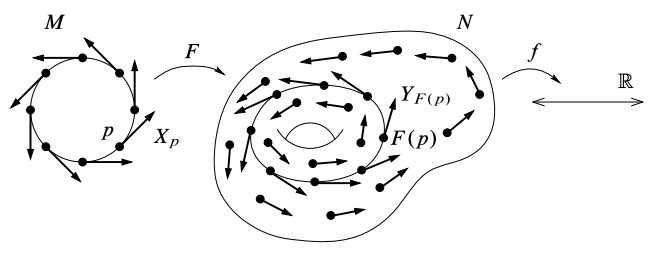
\includegraphics[scale = 0.5]{F_related_vector_fields.png}}
\end{minipage}
\caption{\footnotesize{\textbf{$F$-related vector fields \citep{lee2003introduction}}}}
\label{fig: F_related_vector_fields}
\end{figure}

\item 
\begin{definition}
Suppose $F: M \rightarrow N$ is \emph{smooth} and $X$ is a \emph{vector field} on $M$,  and suppose there happens to be a \emph{vector field} $Y$ on $N$ with the property that for each $p \in M$,
\begin{align*}
dF_{p}(X_p) &= Y_{F(p)}.
\end{align*}
 In this case, we say \emph{the \textbf{vector fields} $X$ and $Y$ are \underline{\textbf{F-related}}} (see Fig. \ref{fig: F_related_vector_fields}). 
\end{definition}

\item \begin{remark}
The \emph{\textbf{differential}} $dF_{p}$ is defined \emph{locally}, and it \emph{\textbf{does not guarantee to map a vector field (a global concept) to a vector field}}.  For example,
if $F$ is \emph{not surjective}, there is no way to decide what vector to assign to a point $q \in N \setminus F(M)$.  If $F$ is \emph{not injective}, then for some points of $N$ there may be several different vectors obtained by applying $dF$ to $X$ at different points of $M$.
\end{remark}

\item \begin{proposition}
Suppose $F: M \rightarrow N$ is a smooth map between manifolds with or without boundary, $X \in \mathfrak{X}(M)$, and $Y \in \mathfrak{X}(N)$. Then $X$ and $Y$ are \textbf{$F$-related} \textbf{if and only if} for \textbf{every smooth real-valued function} $f$ defined on an open subset of $N$,
\begin{align}
X(f \circ F) &= (Yf) \circ F \label{eqn: F_related_vector_fields_condition}
\end{align}
\end{proposition}
\begin{proof}
For any $p \in M$ and any smooth real-valued $f$ defined in a neighborhood of $F(p)$, 
\begin{align*}
X(f \circ F)(p) &= X_{p}(f \circ F) = dF_{p}(X_{p})(f),
\end{align*} while
\begin{align*}
((Yf) \circ F)(p) &= (Yf)(F(p)) = Y_{F(p)}(f).
\end{align*} Thus, \eqref{eqn: F_related_vector_fields_condition}  is true for all $f$ if and only if $dF_{p}(X_p) = Y_{F(p)}$ for all $p$, i.e., if and
only if $X$ and $Y$ are $F$-related. \qed
\end{proof}

\item 
\begin{proposition}
Suppose $M$ and $N$ are smooth manifolds with or without boundary, and $F: M \rightarrow N$ is a \textbf{diffeomorphism}. For every $X \in \mathfrak{X}(M)$, there is a \textbf{unique} smooth vector field on $N$ that is $F$-related to $X$.
\end{proposition}
\begin{proof}
Note that for  $Y \in \mathfrak{X}(N)$ to be F-related to $X$ means that $dF_{p}(X_p) = Y_{F(p)}$ for every $p \in M$. If $F$ is a \emph{diffeomorphism}, therefore, we define $Y$ by
\begin{align*}
Y_{q} &= dF_{F^{-1}(q)}(X_{F^{-1}(q)}),\quad \forall q\in N.
\end{align*} We can show that $Y$ is  $F$-related to $X$. Note that $Y: N \rightarrow TN$ is the \emph{composition} of the following smooth maps:
\begin{align*}
N \stackrel{F^{-1}}{\longrightarrow} M \stackrel{X}{\longrightarrow} TM \stackrel{dF}{\longrightarrow} TN.
\end{align*} It follows that $Y$ is smooth. \qed
\end{proof}


\item \begin{definition}
Suppose $M$ and $N$ are \emph{smooth manifolds with or without boundary}, and $F: M \rightarrow N$ is a \textbf{\emph{diffeomorphism}}. For every $X \in \mathfrak{X}(M)$, there is a \textbf{\emph{unique}} \emph{smooth vector field} $Y$ on $N$ that is $F$-related to $X$. We denote the \emph{\textbf{unique vector field}} that is \emph{\textbf{$F$-related}} to $X$ by \underline{$F_{*}X$}, and call it the \underline{\emph{\textbf{pushforward of $X$ by $F$}}}. And $F_{*}X$ is defined explicitly by the formula
\begin{align}
(F_{*}X)_{q} &= dF_{F^{-1}(q)}(X_{F^{-1}(q)}),\quad \forall q\in N. \label{eqn: pushforward_of_vector_fields}
\end{align} 
\end{definition}
As long as the inverse map $F^{-1}$ can be computed explicitly, the \emph{\textbf{pushforward}} of a vector field can be computed directly from this formula. Note that sometimes the \emph{pushforward} of $X$ is denoted as $F_{\#}X$.

\item \begin{corollary}
Suppose $F: M \rightarrow N$ is a diffeomorphism and $X \in \mathfrak{X}(M)$.  For any $f \in \cC^{\infty}(N)$, 
\begin{align*}
(F_{*}X\,f) \circ F &= X(f \circ F)
\end{align*}
\end{corollary}
\end{itemize}


\subsection{Vector Fields and Submanifolds}
\begin{itemize}
\item \begin{remark}
If $S \subseteq M$ is an immersed or embedded submanifold (with or without boundary), \emph{a vector field $X$} on $M$ does \emph{\textbf{not necessarily} restrict to a vector field on $S$}, because $X_p$ may not lie in the \emph{subspace} $T_{p}S \subseteq T_{p}M$ at a point $p \in S$.
\end{remark}

\begin{figure}
\begin{minipage}[htb]{1\linewidth}
  \centering
  \centerline{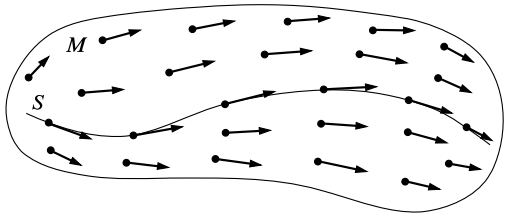
\includegraphics[scale = 0.5]{vector_field_tangent_subman.png}}
\end{minipage}
\caption{\footnotesize{\textbf{A vector field tangent to a submanifold. \citep{lee2003introduction}}}}
\label{fig: vector_field_tangent_subman}
\end{figure}


\item \begin{definition}
Given a point $p \in S$, a vector field $X$ on $M$ is said to \underline{\emph{\textbf{be tangent to}}} $S$ at $p$ if $X_p \in T_{p}S \subseteq T_{p}M$. It \emph{i\textbf{s tangent to}} $S$ if it is tangent to $S$ at every point of $S$.
\end{definition}

\item \begin{proposition}
Let $M$ be a smooth manifold, $S\subseteq M$ be an \textbf{embedded submanifold} with or without boundary, and $X$ be a smooth vector field on $M$. Then $X$ is
\textbf{tangent} to $S$ if and only if $(Xf)|_{S} = 0$ for \textbf{every} \underline{$f \in \cC^{\infty}(M)$}  \textbf{such that} \underline{$f|_{S}\equiv 0$}.
\end{proposition}

\item \begin{remark}
Suppose $S\subseteq M$ is an \textbf{\emph{immersed submanifold}} with or without boundary, and $Y$ is a smooth vector field on $M$. If there is a vector field $X \in \mathfrak{X}(S)$ that is \underline{\emph{\textbf{$\iota$-related to $Y$}}}, where $\iota: S \xhookrightarrow{} M$ is the inclusion map, then clearly \emph{\textbf{$Y$ is tangent to $S$}}, because $Y_p = d\iota_{p}(X_p)$ is in the image of $d\iota_p$ for each $p \in S$. 

The converse is true as well.
\begin{proposition} (\textbf{Restricting Vector Fields to Submanifolds}). \citep{lee2003introduction}\\
Let $M$ be a  smooth manifold, let $S\subseteq M$ be an \textbf{immersed submanifold} with or without boundary, and let $\iota: S \xhookrightarrow{} M$ denote the inclusion map. If $Y \in \mathfrak{X}(M)$ is \textbf{tangent to} $S$, then there is a \textbf{unique smooth vector field} on $S$, denoted by $Y|_{S}$ , that is \textbf{$\iota$-related to $Y$}.
\end{proposition}
\end{remark}
\end{itemize}

\section{Lie Brackets}
\begin{itemize}
\item In this section we introduce an important way of \emph{\textbf{combining} two smooth vector fields} to obtain \emph{another vector field}.

\item \begin{definition}
Let $X$ and $Y$ be smooth vector fields on a smooth manifold $M$ and $f \in \cC^{\infty}(M)$ is smooth function  on $M$. Define an \emph{\textbf{operator}} $[X,Y] : \cC^{\infty}(M) \rightarrow \cC^{\infty}(M)$, called \underline{\emph{\textbf{the Lie bracket}}} of $X$ and $Y$, defined by
\begin{align}
[X,Y]\,f &= XYf - YXf. \label{eqn: lie_bracket}
\end{align}
\end{definition}

\item \begin{remark}
A vector field maps a smooth function on $M$ to another smooth function on $M$. Thus it is valid to define $XYf = Xg$ where $g= Yf$ is the derivation of $f$ under $Y$. $[X, Y]_{p}f$ is \emph{\textbf{a second-order (directional) derivatives}} of $f$ at $p$ along two directions $Y_p$ and $X_p$.
\end{remark}

\item \begin{remark}
Note that $XY$ itself is not a vector field since it does not necessarily satisfy the Leibnitz rule. For example, $X = \partdiff{}{x}$ and $Y = x \partdiff{}{y}$. Let $f(x, y) = x$ and $g(x, y) = y$. Then direct computation shows that $XY(fg) = 2x$, while $f XYg + g XYf  = x$, so $XY$ is not a derivation of $\cC^{\infty}\bR^2$.
\end{remark}

\item \begin{lemma}
The \textbf{Lie bracket} of \textbf{any pair} of smooth vector fields is a smooth vector field.
\end{lemma}
\begin{proof}
It suffices to show that $[X,Y]$ is a \emph{derivation} of $\cC^{\infty}(M)$. For arbitrary $f, g \in \cC^{\infty}(M)$, we compute
\begin{align*}
[X,Y](fg) &= XY(fg) - YX(fg) \\
&= X(f\,Y(g) + g\,Y(f)) - Y(f\,X(g) + g\,X(f)) \\
&= f\,XY(g) + g\,XY(f) - f\,YX(g) - g\,YX(f) \\
&= f\,(XY - YX)(g) + g\,(XY - YX)(f)  \\
&= f\,[X, Y](g) + g\,[X, Y](f). \qed
\end{align*}
\end{proof}

\item \begin{remark}
The \textit{\textbf{value}} of the vector field $[X,Y]$ at a point $p \in M$ is the \emph{derivation at p} given
by the formula
\begin{align}
[X, Y] _{p}f &=  X_{p}(Yf)- Y_{p}(Xf). \label{eqn: lie_bracket_at_point}
\end{align} However, this formula is of limited usefulness for computations, because it requires one to compute terms involving \emph{second derivatives} of $f$ that will always cancel each other out. 
\end{remark}


\item \begin{proposition} (\textbf{Coordinate Formula for the Lie Bracket}). \citep{lee2003introduction} \\
Let $X, Y$ be smooth vector fields on a smooth manifold $M$ with or without boundary, and let $X = X^i\,\partdiff{}{x^{i}}$ and $Y = Y^j\partdiff{}{x^{j}}$ be the coordinate expressions for $X$ and $Y$ in terms of some smooth local coordinates $(x^i)$ for $M$. Then $[X, Y]$ has the following coordinate expression:
\begin{align}
[X, Y]&= \paren{X^{i}\partdiff{Y^{j}}{x^{i}} - Y^{i}\partdiff{X^{j}}{x^{i}} }\partdiff{}{x^{j}},  \label{eqn: lie_bracket_coordinate}
\end{align} or more concisely,
\begin{align}
[X, Y]&= \paren{XY^{j}  - YX^{j}}\partdiff{}{x^{j}}.  \label{eqn: lie_bracket_coordinate_2}
\end{align}
\end{proposition}

\item \begin{remark} One trivial application of \eqref{eqn: lie_bracket_coordinate_2} is to compute the Lie brackets of the coordinate
vector fields $\partdiff{}{x^{i}}$  in any smooth chart: because \emph{the component functions} of \emph{the coordinate vector fields} are \emph{all constants}, it follows that
\begin{align}
\brac{\partdiff{}{x^{i}},  \partdiff{}{x^{j}}}&\equiv 0, \quad \forall\, i,j.  \label{eqn: lie_bracket_coordinate_vector_fields}
\end{align} 

This also follows from the definition of the Lie bracket, and is essentially a restatement of the fact that \emph{\textbf{mixed partial derivatives of smooth functions commute}}.
\end{remark}

\item \begin{proposition} (\textbf{Properties of the Lie Bracket}). \\
The \textbf{Lie bracket} satisfies the following identities for all $X, Y, Z \in \mathfrak{X}(M)$:
\begin{enumerate}
\item \underline{\textbf{Bilinearity}}:  For $a,b \in \bR$, 
\begin{align*}
[aX +bY, Z] &= a[X, Z] + b [Y, Z], \\
[Z, aX + bY] &= a[Z, X] + b[Z, Y].
\end{align*}
\item \underline{\textbf{Antisymmetry}}:
\begin{align*}
[X, Y] &= - [Y, X]
\end{align*}
\item \underline{\textbf{Jacobi Identity}}:
\begin{align*}
[X, [Y, Z]] + [Y, [Z, X]] + [Z, [X, Y]]&= 0 
\end{align*}
\item For $f, g \in \cC^{\infty}(M)$, 
\begin{align}
[fX, gY] &= fg [X, Y] + (fXg)\, Y - (gYf)\,X \label{eqn: lie_bracket_scale_by_fun}
\end{align}
\end{enumerate}
\end{proposition} 

The significance of part 4 of this proposition might not be evident at this point, but it will become clearer in the next chapter, where we will see that it expresses the
fact that the \emph{\textbf{Lie bracket}} satisfies \emph{product rules} with respect to \emph{\textbf{both of its arguments}}.

\item  \begin{proposition} (\textbf{Naturality of the Lie Bracket}). \citep{lee2003introduction} \\
Let $F: M \rightarrow N$ be a smooth map between manifolds with or without boundary, and let $X_1, X_2\in \mathfrak{X}(M)$ and
$Y_1, Y_2\in \mathfrak{X}(N)$ be \textbf{vector fields} such that $X_i$ is \textbf{$F$-related to} $Y_i$ for $i= 1,2$. Then $[X_1, X_2]$ is \textbf{$F$-related to} $[Y_1, Y_2]$.
\end{proposition}
\begin{proof} Using the fact that $X_i$ and $Y_i$ are $F$-related, for $f \in \cC^{\infty}(M)$, $X_i(f\circ F) = (Y_i f) \circ F$ for $i=1,2$. Thus
\begin{align*}
[X_1, X_2](f \circ F) &= X_1X_2(f \circ F) - X_2X_1(f \circ F)\\
&= X_1((Y_2 f) \circ F) - X_2((Y_1 f) \circ F) \\
&= Y_1 Y_2 f \circ F - Y_2 Y_1 f \circ F\\
&= ([Y_1, Y_2] f ) \circ F.
\end{align*} So $[X_1, X_2]$ is \textbf{$F$-related to} $[Y_1, Y_2]$. \qed
\end{proof}

\item \begin{corollary} (\textbf{Pushforwards of Lie Brackets}). \\
Suppose $F: M \rightarrow N$ is a \textbf{diffeomorphism} and $X_1, X_2\in \mathfrak{X}(M)$. Then 
\begin{align*}
F_{*}[X_1, X_2] = [F_{*}X_1,  F_{*} X_2].
\end{align*}
\end{corollary}

\item \begin{corollary} (\textbf{Brackets of Vector Fields Tangent to Submanifolds}). \\
Let $M$ be a smooth manifold and let $S$ be an \textbf{immersed submanifold} with or without boundary in $M$. If $Y_1$ and $Y_2$ are smooth vector fields on $M$ that are \textbf{tangent} to $S$, then $[Y_1, Y_2]$ is also \textbf{tangent} to $S$.
\end{corollary}
\end{itemize}

\section{The Lie Algebra of a Lie Group}
\subsection{Lie Algebra}

\subsection{Induced Lie Algebra Homomorphisms}

\subsection{The Lie Algebra of a Lie Subgroup}


\newpage
\bibliographystyle{plainnat}
\bibliography{book_reference.bib}
\end{document}